\documentclass[a4paper,12pt]{article}

\usepackage{amsmath,amssymb}
\usepackage{graphicx,float,subcaption}
\usepackage[margin=1in]{geometry}

\title{Notes on spin-wave analysis}
\author{Yang Yang}

\begin{document}
	\maketitle
	\section{Spin wave on the Heisenberg ferromagnet}
		For the Heisenberg ferromagnet, we consider a constant Heisenberg ferromagnetic interaction $J$ between any spin pairs, so the ground state of the system consists of spins aligning parallel to each other, independent from the geometrical structure of the lattice, and hence we have the Hamiltonian
		\begin{align}
			\mathcal{H}&=J\sum_{\langle i,j \rangle}\mathbf{S}_i\cdot\mathbf{S}_j\nonumber\\
			&=J\sum_{\langle i,j \rangle}
			\label{equ:h1}\left(S_i^xS_j^x+S_i^yS_j^y+S_i^zS_j^z\right)
		\end{align}
		with $J<0$. When we adapt the linear expansion of Holstein-Primakoff(HP) transformation
		\begin{align}
			S^+&=\sqrt{2S}\sqrt{1-\frac{a^\dagger a}{2S}}a\approx\sqrt{2S}a\\
			S^-&=\sqrt{2S}a^\dagger\sqrt{1-\frac{a^\dagger a}{2S}}\approx\sqrt{2S}a^\dagger,
		\end{align}
		we have 
		\begin{align}
			S^x&\approx\sqrt{\frac{S}{2}}(a+a^\dagger)\\
			S^y&\approx-i\sqrt{\frac{S}{2}}(a-a^\dagger)
		\end{align}
		Along with
		\begin{align}
			S^z=S-a^\dagger a,
		\end{align}
		we obtain the linear spin wave Hamiltonian from (\ref{equ:h1}) in HP bosons operators
		\begin{align}
			\mathcal{H}=J S\sum_{\langle i,j \rangle}(a_ia_j^\dagger+a_i^\dagger a_j-a_i^\dagger a_i-a_j^\dagger a_j)
		\end{align}
		After performing Fourier transform
		\begin{align}
			a_i&=\frac{1}{\sqrt{N}}\sum_{\mathbf{k}}e^{i\mathbf{k}\cdot\mathbf{r}_i}a_\mathbf{k}\\
			a_i^\dagger&=\frac{1}{\sqrt{N}}\sum_{\mathbf{k}}e^{-i\mathbf{k}\cdot\mathbf{r}_i}a_\mathbf{k}^\dagger\label{equ:fourier1},
		\end{align}
		we get
		\begin{align}
			\nonumber
			\mathcal{H}=&JS\sum_{\langle i,j\rangle}\sum_{\mathbf{k}}\sum_{\mathbf{k'}}\\&\frac{1}{N}(e^{i\mathbf{k}\cdot\mathbf{r}_i}e^{-i\mathbf{k}'\cdot\mathbf{r}_j}a_\mathbf{k}a_{\mathbf{k}'}^\dagger +e^{-i\mathbf{k}\cdot\mathbf{r}_i}e^{i\mathbf{k}'\cdot\mathbf{r}_j}a_\mathbf{k}^\dagger a_{\mathbf{k}'}-e^{-i\mathbf{k}\cdot\mathbf{r}_i}e^{i\mathbf{k}'\cdot\mathbf{r}_i}a_\mathbf{k}^\dagger a_{\mathbf{k}'}-e^{-i\mathbf{k}\cdot\mathbf{r}_j}e^{i\mathbf{k}'\cdot\mathbf{r}_j}a_\mathbf{k}^\dagger a_{\mathbf{k}'}).
			\label{equ:h3}
		\end{align}
		Noticing for every geometrical structure, we can regard index $i$ running through every lattice site and index $j$ as all the nearest neighboring sites around $i$, we can rewrite
		\begin{align}
			\mathbf{r}_j=\mathbf{r}_i+\mathbf{\Delta}_j,
			\label{equ:local}
		\end{align}
		where $\mathbf{\Delta}_j$ is defined as a local position vector pointing towards neighboring lattice site $j$ from site $i$.
		\begin{figure}[H]
			\centering
			\begin{subfigure}[b]{0.3\textwidth}
				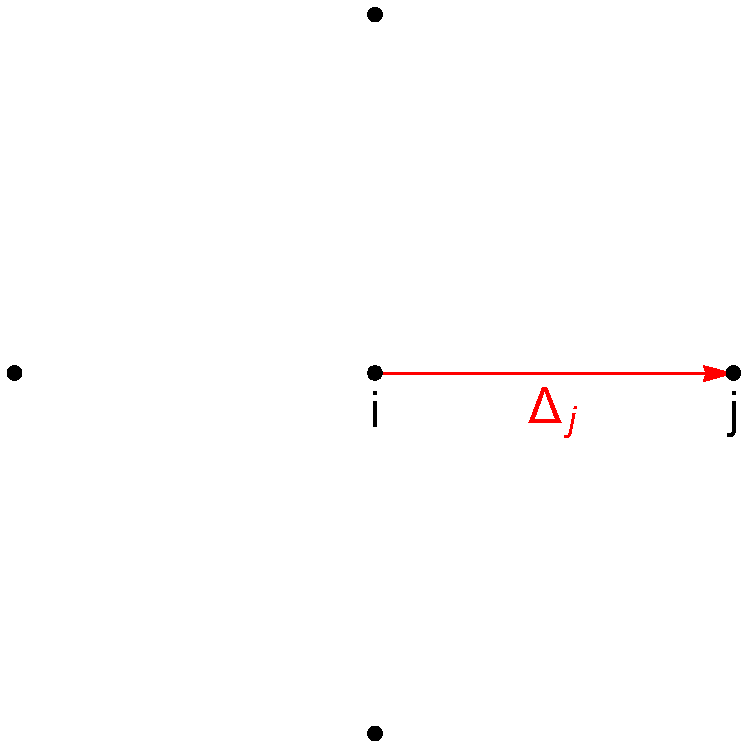
\includegraphics[width=4cm,keepaspectratio]{sq_local}
				\caption{Square lattice}
				\label{fig:sq_local}
			\end{subfigure}
			\quad
			\begin{subfigure}[b]{0.3\textwidth}
				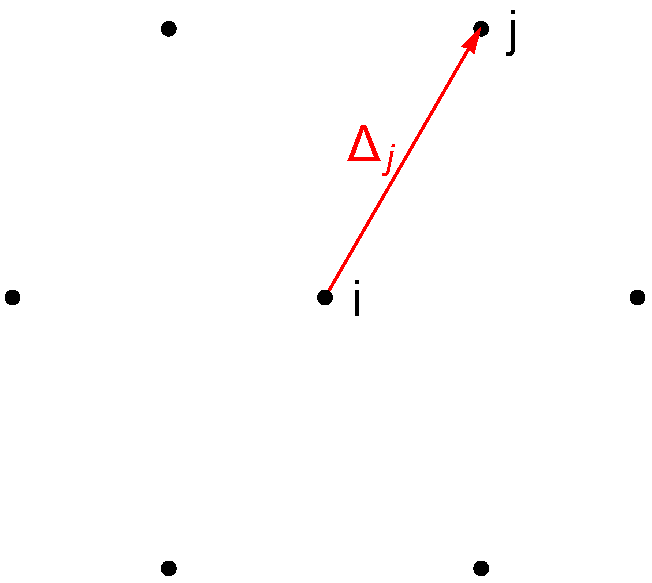
\includegraphics[width=4cm,keepaspectratio]{tri_local}
				\caption{Triangular lattice}
				\label{fig:tri_local}
			\end{subfigure}
			\caption{Nearest neighbors on the square and triangular lattice with their corresponding local position vector $\mathbf{\Delta}_j$}
		\end{figure}
		Then we can substitute (\ref{equ:h3}) with (\ref{equ:local}), and get 
		\begin{align}
			\mathcal{H}=\frac{JS}{2N}\sum_{i,j,\mathbf{k},\mathbf{k}'}\left[e^{i(\mathbf{k}-\mathbf{k}')\cdot\mathbf{r}_i}e^{-i\mathbf{k}'\cdot\mathbf{\Delta}_j}a_\mathbf{k}a^\dagger_{\mathbf{k}'}+e^{-i(\mathbf{k}-\mathbf{k}')\cdot\mathbf{r}_i}\left(e^{i\mathbf{k}'\cdot\mathbf{\Delta}_j}-1-e^{-i(\mathbf{k}-\mathbf{k}')\cdot\mathbf{\Delta}_j}\right)a_\mathbf{k}^\dagger a_{\mathbf{k}'}\right].
		\end{align}
		With 
		\begin{align}
			\sum_{i}e^{i(\mathbf{k}-\mathbf{k}')\cdot\mathbf{r}_i}&=N\delta_{\mathbf{k},\mathbf{k}'}\\
			\sum_{\mathbf{k}}e^{-i\mathbf{k}\cdot\mathbf{\Delta}_j}&=0
		\end{align}
		we have 
		\begin{align}
			\mathcal{H}&=\frac{JS}{2}\sum_{j,\mathbf{k}}\left[e^{-i\mathbf{k}\cdot\mathbf{\Delta}_j}a_\mathbf{k}a^\dagger_{\mathbf{k}}+\left(e^{i\mathbf{k}\cdot\mathbf{\Delta}_j}-2\right)a_\mathbf{k}^\dagger a_{\mathbf{k}}\nonumber\right]\\
			&=\frac{JS}{2}\sum_{j,\mathbf{k}}\left[\left(2\cos(\mathbf{k}\cdot\mathbf{\Delta}_j)-2\right)a_\mathbf{k}^\dagger a_{\mathbf{k}}+e^{-i\mathbf{k}\cdot\mathbf{\Delta}_j}\right]\nonumber\\
			&=JS\sum_{\mathbf{k}}(\gamma(\mathbf{k})-n)a_\mathbf{k}^\dagger a_{\mathbf{k}},\label{equ:ferro_dispersion}
		\end{align}
		where we define $\gamma(\mathbf{k})=\sum_{j}\cos(\mathbf{k}\cdot\mathbf{\Delta}_j)$ and $n$ the number of nearest neighbors.
		
		It is clear from (\ref{equ:ferro_dispersion}) that geometrical structure of lattice sites enters the dispersion relation only through the geometric factor $\gamma(\mathbf{k})$. Hence for different lattice configuration, we only need to find the corresponding $\gamma(\mathbf{k})$. For square lattice and triangular lattice with lattice constant $a=1$, we have 
		\begin{align}
			\gamma_{\text{sq}}(\mathbf{k})&=2\left[\cos(k_x)+\cos(k_y)\right]\\
			\gamma_{\text{tri}}(\mathbf{k})&=2\left[\cos(k_x)+\cos\left(\frac{k_x}{2}-\frac{\sqrt{3}}{2}k_y\right)+\cos\left(\frac{k_x}{2}+\frac{\sqrt{3}}{2}k_y\right)\right].
		\end{align}
		Therefore, we can get energy dispersion relation for linear spin wave on both lattices by substituting corresponding $\gamma(\mathbf{k})$ in
		\begin{align}
			w(\mathbf{k})=|JS|(n-\gamma(\mathbf{k})).
		\end{align}
				\begin{figure}[H]
			\centering
			\begin{subfigure}[b]{0.4\textwidth}
				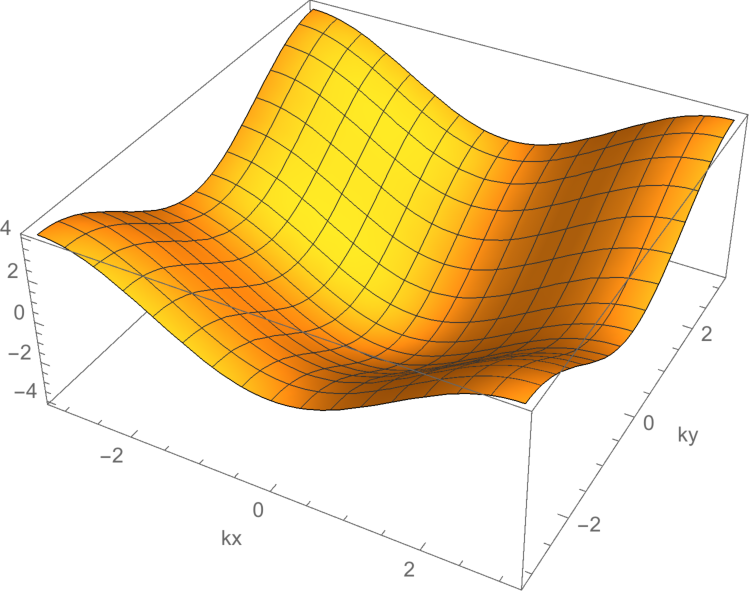
\includegraphics[width=6cm,keepaspectratio]{sq_dispersion}
				\caption{$w(\mathbf{k})$ for square lattice }
				\label{fig:sq_dispersion}
			\end{subfigure}
			\quad
			\begin{subfigure}[b]{0.4\textwidth}
				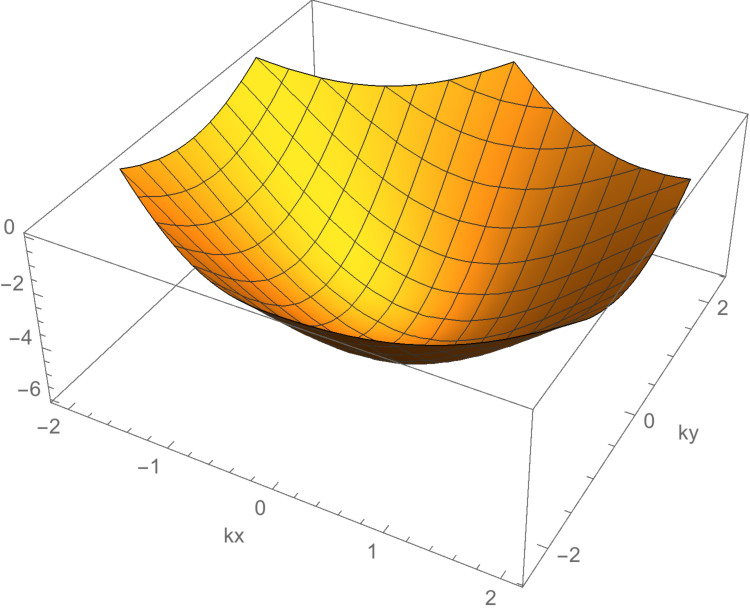
\includegraphics[width=6cm,keepaspectratio]{tri_dispersion}
				\caption{$w(\mathbf{k})$ for triangular lattice }
				\label{fig:tri_dispersion}
			\end{subfigure}
			\caption{Energy dispersion relation for linear spin wave on the square and triangular lattice}
		\end{figure}
	\section{Spin wave on the Heisenberg Antiferromagnet}
\end{document}